\chapter{人类移动性}

移动性其实分为很多种,人类移动性、商品的移动性、信息的移动性都被研究了很多。Physics Reports 有一篇综述,\href{https://www.sciencedirect.com/science/article/pii/S037015731830022X}{Human mobility: Models and applications}

\section{经典模型}

王铮老师有一本书大家可以看一下,叫《理论经济地理学》里面有大量的地理学模型。虽然不算新,也没有什么实证分析,不过想法很值得借鉴。

\subsection{重力模型}

重力模型可能是地理学中最有名的模型了。形式如下:\begin{equation}
T_{i j}=\frac{m_{i}^{\alpha} n_{j}^{\beta}}{f\left(r_{i j}\right)}
\end{equation}

重力模型对火车运货量\href{https://www.jstor.org/stable/2087063?origin=crossref}{Zipf, G. K. The P 1P 2/D hypothesis: On the intercity movement of persons. Am. Sociol. Rev. 11, 677–686 (1946).}、地铁乘客\href{https://journals.aps.org/pre/abstract/10.1103/PhysRevE.86.026102}{Goh, S., Lee, K., Park, J. S. and Choi, M. Y. Modification of the gravity model and application to the metropolitan Seoul subway system. Phys. Rev. E 86, 026102 (2012).}、韩国高速公路\href{https://iopscience.iop.org/article/10.1209/0295-5075/81/48005}{Jung, W. S., Wang, F. and Stanley, H. E. Gravity model in the Korean highway. EPL 81, 48005 (2008).}、航空网络\href{https://doi.org/10.1016/j.jairtraman.2007.02.001}{Grosche, T., Rothlauf, F. and Heinzl, A. Gravity models for airline passenger volume estimation. J. Air Transp. Manag. 13, 175–183 (2007).}、通勤\href{https://science.sciencemag.org/content/312/5772/447}{Viboud, C. et al. Synchrony, waves, and spatial hierarchies in the spread of influenza. Science 312, 447–451 (2006).}和人口迁移\href{https://www.tandfonline.com/doi/abs/10.2747/0272-3638.16.4.327}{Tobler, W. Migration: Ravenstein, thornthwaite, and beyond. Urban Geogr. 16, 327–343 (1995).}等问题的拟合很不错。

通过目的地选择来推导重力模型是一个学术套路,我觉得还能玩二十年。目前目的地选择的理论有这样一些根源:确定性效用理论\href{https://doi.org/10.1111/j.1467-9787.1969.tb01340.x}{Niedercorn, J. H. and Bechdolt, B. V. Jr. An economic derivation of the "gravity law” of spatial interaction. J. Regional Sci. 9, 273–282 (1969).}、随机效用理论\href{https://www.jstor.org/stable/134305?origin=crossref}{Domencich, T. A. and  Mcfadden, D. Urban travel demand: A behavioral analysis. (North-Holland, Amsterdam, 1975).}、博弈论\href{https://www.nature.com/articles/s41598-019-46026-w}{Yan, X. Y. and Zhou, T. Destination choice game: A spatial interaction theory on human mobility. Sci. Rep. 9, 1–9 (2019).}等。文章最近也还有,不过都是集中在SR之类的期刊上。

\begin{quote}
    一个规律如果基本是客观存在且不很精确的话,不同的发现方法总是能发出文章的。毕竟人类对于规律的探索就像对孤独的回避。
\end{quote}
  
\subsection{辐射模型/介入机会(IO)模型}

辐射模型记载在Simini和Marta等人一篇名声不大好的Nature论文里,\href{https://www.nature.com/articles/nature10856}{A universal model for mobility and migration patterns. Nature 484, 96–100 (2012).}

文章中的配图甚是有意思,图一小人的表情是有出处的。法国大作家雨果写毕名著《巴黎圣母院》,与出版商有了这番史上最短通信:
\begin{center}
    “?—雨果”\\
    “!—出版商”
\end{center}

辐射模型刻画了:

辐射模型的表述如下:\begin{equation}
\left\langle T_{i j}\right\rangle=T_{i} \frac{m_{i} n_{j}}{\left(m_{i}+s_{i j}\right)\left(m_{i}+n_{j}+s_{i j}\right)}
\end{equation}其中,$T_{ij}$表示$i$到$j$的流量,$m_i$,$n_j$代表两个位置的人口,$r_{ij}$为两地距离,$s_{ij}$代表以$i$为中心,$r_{ij}$为半径的圆内的人口总数。

严小勇同志又搞了一篇Scientific Reports,\href{https://doi.org/10.1038/s41598-020-61613-y}{Liu, E., Yan, X. A universal opportunity model for human mobility. Sci Rep 10, 4657 (2020). } 介入机会(intervening opportunity)\footnote{\href{https://www.baidu.com/link?url=x-lW8LLAwVj0UCSvfYwmmsvSsLs4MiNoFonbejPvLVbktEM5xeFK2-0nwgOvZprl&wd=&eqid=b1f1d8ba0007275e000000035e8c3a1e}{Stouffer, S. A. Intervening opportunities: A theory relating mobility and distance. Am. Sociol. Rev. 5, 845–867 (1940).}}模型说的是:个体选择目的地与两个因素相关,终点的机会与起点终点之间介入的机会(?)。此类模型可以给出特定时空尺度上的准确预测,但是不同尺度上都合适的IO模型在上面这篇文章是第一次给出的。本文考虑的是人类行为的两个倾向:探索倾向和谨慎倾向。模型的形式是\begin{equation}
    {Q}_{ij}={\int }_{0}^{\infty }{\Pr }_{{m}_{i}+\alpha \cdot {s}_{ij}}(z){\Pr }_{\beta \cdot {s}_{ij}}( < z){\Pr }_{{m}_{j}}( > z)dz,
\end{equation}

\section{有意思的工作}

这个工作可以作为Allee工作的基础。

\begin{itemize}
    \item 数据源:2006年48个加拿大城市通勤普查数据,总共7 225 810人。每个城市的数据按照 census tract 组织,记录了每对职住地的人口数为$T_{ij}$. 每个 CT 约有2500-8000人居住,一般是一个城市的数个街区的大小。
\end{itemize}

CT 边界与有多少人选该CT作为工作地没有关系。记$n_{ij} = \sum_j T_{ij}$, $m_{ij} = \sum_i T_{ij}$. 将$m_j$看作随机变量,统计特征$\bar{m}$, $\sigma_m$。$W$是总工人数,$N$是城市总人口。Lloyd的平均聚集统计量:$m^* = \bar{m} + \sigma^2_m/\bar{m} - 1$ 从工作地的角度度量了工人的密度,是与随机选一个工人在同一个地方工作的工人的期望数。

\textbf{为了刻画城市间的人类移动性差异},作者动用了辐射模型。模型中,$\langle T_{ij} \rangle = p_{ij} n_{i}$其中$p_{ij}$是人取自$ij$流的概率,$n_{i}$是家处人口。利用~\cite{PhysRevE.66.016128}重的配置模型来采样。

Our model makes two assumptions: first, we assume that the spatial trajectories of humans in cities can be predicted by their home and workplace locations, which is supported by recent analyses of high-resolution data on the relocation patterns of mobile phone users [13]; second, we assume that excursions from an individual's bed or work station are governed by a stochastic process that is identically distributed across cities. 

为了实现模型,
\begin{enumerate}
    \item 先利用通勤数据来估计两地的交互频率。
    \item 将频率翻译成逐对的传播概率 $\lambda: $ the strain-specific ratio between within-hostpathogen load and transmission hazard 
\end{enumerate}

\vspace{1cm}

通勤模式分析:通勤矩阵$T_ij$的结构在城市内部和城市之间都发生了显着变化。这些可视化中的显着特征是某些城市出现了\textbf{星形}。星形形状出现在源自许多不同CT的通勤流被导向单个集中工作位置的地方。拥挤统计量$m^*$可以用来衡量城市中星型通勤模式的发生率,因为它的价值随着各个工作地点的聚集程度而增加。\begin{figure}
    \centering
    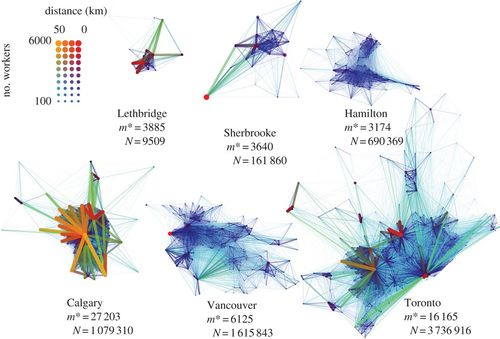
\includegraphics[width = 0.8\linewidth]{Pics/rspb20130763f01.jpg}
    \caption{城市工人的流动方式。边缘的厚度和颜色显示了CT之间上下班的人数。圆圈实际上是短边,代表生活在同一CT中的个人。较大的城市通勤模式往往井井有条,这是通过将工作站与随机选择的工人位于同一CT上的工人的平均人数来衡量的($m^*$)。但是,城市也显示出明显的组织差异,与人口规模无关。}
\end{figure}
随着总人口$N$增加,平均通勤人数$\bar{m}$很快就会饱和。相反的,$m^*$则会显示出与$N$的强烈正相关。说明大城市里的工人更倾向于前往几个巨型的工作地进行工作,但是平均每个CT中的工作地数量跟小城市差不多。所以,星形程度与在CT中工作的平均人数只是弱相关,但是与总人口关系很大。所以大城市在城市中心集中组织的程度更高。

城市还表现出明显的与大小无关的$m^*$变化,这在$m^*$随函数N回归所预测的值之比中很明显(参见电子补充材料,表S2)。在我们分析的48个城市中,$m^*/\bar{m}$(以下称为“流动性模式中的过度异质性”)介于0.43至3.07之间,相差7.14倍。对于随机选择的两个城市,的较大值和较小值之间的平均比率$m^*/\bar{m}$是1.55。在移动性模式这个尺寸无关的差相当于所预测的大小依赖性差异(基于图~\ref{rspb20130763f02} 一个),这将导致从人口尺寸的2.64倍的变化。因此,与人口规模无关的差异是城市之间工人流动模式差异的重要组成部分。
\begin{figure}
    \centering
    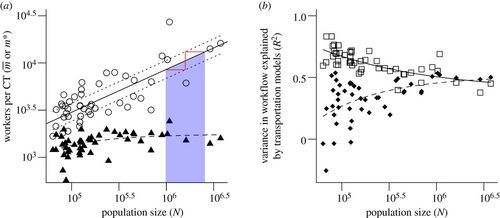
\includegraphics[width = 0.8\linewidth]{Pics/rspb20130763f02.jpg}
    \caption{Variance explained in each city by the configuration (squares) and radiation (diamonds) models of commuting flows.}
    \label{rspb20130763f02}
\end{figure}
配置模型解释了小城市通勤流量的大部分变化,但是随着N的增加,其性能会系统地下降,这表明大城市的交通方式组织化程度越来越高(图2b)。引力模型的拟合度比配置模型的拟合度差,但与大城市相比,它表现出与较小的城市更好拟合的相同趋势(请参阅电子补充材料)。辐射模型还显示出性能的系统变化:随着配置模型的适合度下降,辐射模型的性能增加,在小城市中表现相对较差,而在大城市中则更好(图2b)。

$m^*$更大代表更有条理。